% threedbox.tex
%https://texample.net/tikz/examples/sudoku-3d-cube/
\documentclass[12pt]{article}
\usepackage{tikz}
\usetikzlibrary{positioning}
\begin{document}
\large
\pagestyle{empty}
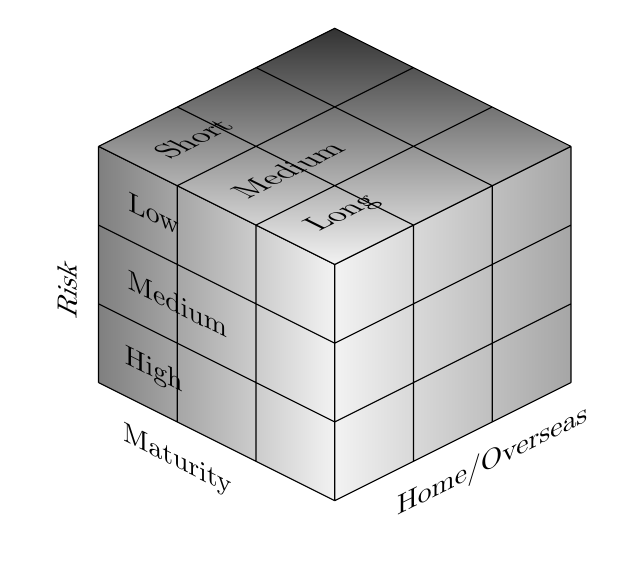
\begin{tikzpicture}[every node/.style={minimum size=1cm},on grid]
\begin{scope}[every node/.append style={yslant=-0.5},yslant=-0.5]
  \shade[right color=gray!10, left color=black!50] (0,0) rectangle +(3,3);
  \node at (0.7,2.5) {Low};
  \node at (1.5,2.5) {};
  \node at (2.5,2.5) {};
  \node at (1.0,1.5) {Medium};
  \node at (1.5,1.5) {};
  \node at (2.5,1.5) {};
  \node at (0.7,0.5) {High};
  \node at (1.5,0.5) {};
  \node at (2.5,0.5) {};
  \node at (1.0, -0.5) {Maturity};
  \node [rotate=90] at (-0.4, 1.0) {Risk};
  \draw (0,0) grid (3,3);
\end{scope}
\begin{scope}[every node/.append style={yslant=0.5},yslant=0.5]
  \shade[right color=gray!70,left color=gray!10] (3,-3) rectangle +(3,3);
  \node at (3.5,-0.5) {};
  %\node at (4.5,-0.5) {};
  \node at (5.5,-0.5) {};
  \node at (3.5,-1.5) {};
  %\node at (4.5,-1.5) {};
  \node at (5.5,-1.5) {};
  \node at (3.5,-2.5) {};
  %\node at (4.5,-2.5) {};
  \node at (5.5,-2.5) {};
  \node at (5.0,-3.5) {Home/Overseas};
  \draw (3,-3) grid (6,0);
\end{scope}
\begin{scope}[every node/.append style={
    yslant=0.5,xslant=-1},yslant=0.5,xslant=-1
  ]
  \shade[bottom color=gray!10, top color=black!80] (6,3) rectangle +(-3,-3);
  \node at (3.7,2.5) {Short};
  \node at (3.9,1.5) {Medium};
  \node at (3.7,0.6) {Long};



  \node at (3.5,0.5) {};
  \node at (4.5,2.5) {};
  \node at (4.5,1.5) {};
  \node at (4.5,0.5) {};
  \node at (5.5,2.5) {};
  \node at (5.5,1.5) {};
  \node at (5.5,0.5) {};
  \draw (3,0) grid (6,3);
\end{scope}
\end{tikzpicture}
\end{document}